\section{Pre-Concentration Software}

The pre-concentration system is controlled by a Raspberry Pi 3B (Pi) that interfaces with individual control boards either through USB or the GPIO pins. The main program to run the pre-concentration system is located on the Pi in the \code{NMHC-Pre-Concentration} folder. This section covers how to connect to the Pi, and details how to run the pre-concentration system software.

The pre-concentration controller has four levels of hardware control, ranked lowest- to highest-level: individual controls, states, methods, and sequences. Individual control is the direct line that connect the control board to individual components (e.g., switching a valve). Machine states are the combination of all individual controls which generally lock the system in a specified state until a specified \emph{condition} is satisfied, such as waiting a specified amount of time. Methods are a collection of states in a defined order that perform a complete system cycle (e.g., sample 600 mL of air). Sequences are then a collection of methods that run in order. An example of a sequence would include a method to run a calibration standard, followed by multiple sample methods. A map of this behavior is shown in \figref{fig: hardware abstract}
\warn{Each function generally uses the same named function for reading or writing. Getting current values is commonly achieved by using a blank call to a function (e.g., \code{function()}) whereas setting the hardware requires an input to the function (e.g., \code{function(inputs)}). Future updates should consider removing this behavior in favor of get\_(function) and set\_(function) to help avoid accidentally triggering a hardware change.}

\begin{figure}[H]
    \centering
    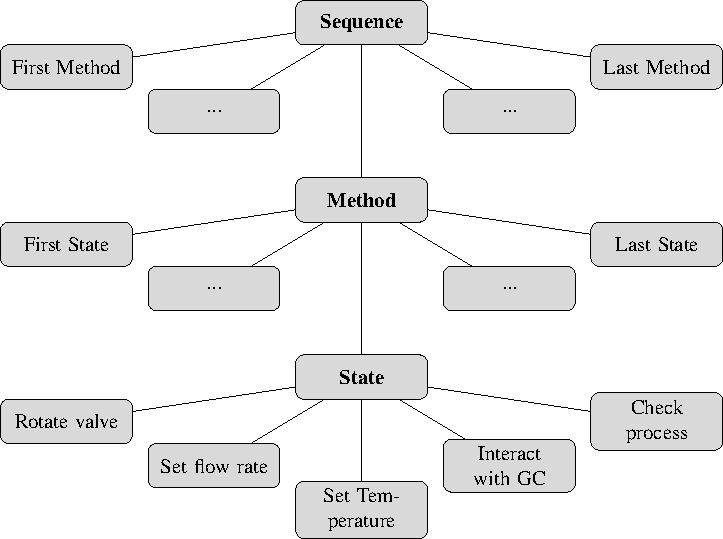
\includegraphics{tikz/Hardware Abstraction.pdf}
    \caption{Map of the four levels of hardware abstraction in the pre-concentration software.}
    \label{fig: hardware abstract}
\end{figure}

\subsection{Remote Desktop Connection}
The Raspian OS installed on the Pi allows for a desktop GUI interface. A keyboard, mouse, and monitor can be connected to the Pi directly, but this can add unnecessary additional hardware. The Pi OS also includes a copy of RealVNC which allows for a remote desktop connection. The connecting computer just needs to install a copy of the RealVNC viewer to access the Pi. Opening a remote desktop connection will create a login instance on the Pi. This allows the remote PC to disconnect without interrupting any actions being performed on the Pi.

The pre-concentration software can be viewed a run from the Thonny IDE. Click the raspberry icon, then navigate to \say{Programming} and open Thonny. The main program is saved under \emph{NMHC-Pre-Concentration/pre\_con.py}. 
This code contains the \code{pre\_con} class. Running it directly will connect the Pi will initialize the \code{pre\_con} class under the name \code{pc}. All pre-concentration functions can be called in the command window using \code{pc.(function)}. These functions are described in detail in the next section.
\warn{RealVNC sessions have been known to timeout. It is not recommended to run extended sequences (24 hrs+) using the Thonny IDE.}

\subsection{Command Line Interfacing}
The command line interface can be accessed using a Secure Shell Protocol (SSH) connection. To SSH into the Pi, open an application like \emph{putty}, or MobaXterm on a computer that is connected to the same local network. Choose an SSH connection that targets the IP address of the PI. If you're using a computer that supports local hostnames (i.e., MacOS or Apple Bonjour is installed on Windows), you can address \emph{raspberrypi.local}. % Add links to putty & mobaxterm
Once you connect, you will be prompted for a username and password (defaults are username: pi, password: password). 
Navigate to the software folder using the command \code{CD NMHC-Pre-Concentration}. 
Once here, you can run the software using the command \code{python pre\_con.py --opt}. \textbf{Warning: any SSH commands will terminate if the connection is interrupted. See \hyperref[auto operation]{Autonomous Operation}.} % Add reference

Running the command line causes the software to initialize the system. It begins by connecting to each subsystem, and setting the pre-concentration system into the default \say{off} state. The software then interprets the options selected and calls the appropriate function. Options for the command line interface are be displayed using \code{-h}, or \code{--help}. The main options for selecting a routine are \code{-r, --run}, and \code{-c, --CLI}.

Additional options are \code{--run} specify pre-concentration conditions (see standard\_method for more). Performing a run from the command line can be specified with the following options: % Add reference to standard method
\begin{itemize}
    \item \code{-{}-volume XXX} - sample volume in milliliters (mL).
    \item \code{-{}-flow XXX} - flow rate in milliliters per minutes (mL/min, sccm).
    \item \code{-{}-temp XXX} - trap temperature in celsius (°C).
    \item \code{-{}-inject XXX} - injection time in seconds (s).
    \item \code{-{}-delay XXX} - amount of time to pause between runs in minutes (min).
    \item \code{-{}-stream N} - selecting sample stream to use on the 16 port-valve .
    \item \code{-{}-repeat} - number of times to repeat a measurement.
    \item \code{-{}-blank} - perform a blank run that \say{samples} the carrier gas.
\end{itemize}
Once the system has completed the run(s) specified, the Pi will disconnect from each subsystem and return to the system command line.

Using the programs CLI (opt \code{-c}) will initialize the pre-concentration system and allow for general user inputs. This allows the operator to access all functionality of the pre-concentration software, and enables the manual override switches. To return to the system command line, the operator simply needs to use the command \code{exit}. The remainder of this chapter describes each function that can be used with the pre-concentration system's CLI.
\warn{When using RealVNC and running the software in a python IDE, the functions are accessed the same way as they are in the CLI, but all function are embedded the object \code{pc}. In the CLI, the object is called directly and evaluated as python code. Thus, running the IDE will require the user to include the prefix \code{pc.} (e.g., instead of \code{valve(1, 1)}, the operator will need to use \code{pc.valve(1,1)} in the python IDE.)}

\subsection{Direct Controls}
Direct controls manipulation the objects attached to the control board: valve controller, mass flow controller, adsorbent trap, water trap, gas chromatograph, and manual override inputs. These functions provided the lowest level of control by directly accessing a specific machine parameter.

\emph{Valve Controller}\\
The valve controller is an ESP32 programmed with micropython to control relays that rotate the rotary valves, apply power to turn on/off the switching valve, and turn the vacuum pump on and off. It also uses a darlington array to communicate with a multi-port selector valve. The simplest control is the pump where it is turned on/off with the command \code{pump(0)}, or \code{pump(1)}. See \ref{VC code} and \figref{fig: valve controller} for details about how the valve controller works.

Valves are turned on/off by using the command \code{valve(valve, position)}. The command will accept a single valve position, a list of valves with a corresponding list of positions, or a list of positions. For a single valve rotation, suppose that valve 0 is turns to the inject position. The rotation is achieved by using the \code{valve(0, 1)}. For changing multiple valves, suppose the system is being prepared to be back flushed. This may require rotating the trap orientation, and activating the back-flush 3-way valve. This is accomplished by using the command \code{valve([2,3], [1,1]}. Alternatively, suppose each other valve is already known. The same two valve rotation can be achieved with the command \code{valve(position=[0, 0, 1, 1, 0])}. Machine states are always defined using the last example.

The valve controller has a built-in command for a more precise timed rotation. This rotates a single valve, and returns to the previous position after the set amount of time (e.g., injecting a specified volume of gas). This is used primarily for sampling to ensure consistency from run to run by having a valve controller time the rotation. This also allows the control board to do other tasks while the valve is being timed. This is done using the command \code{pulse(valve, sleep)}, where \code{sleep} is the amount of time in minutes.

\emph{Mass Flow Controller}\\
Mass flow controls are simplified on the control board side, as there are only commands that set the flow rate on either mass flow controller (MFC). See \ref{Mass Flow Controller} for more information about the MFC controller. Both MFCs (sample and backflush) can be accessed using the command \code{flowrate(index, flow)}, or directly using \code{sampleFlow(flowrate)} or \code{backflush(flowrate)}. The latter commands will use the \code{flowrate} with the proper index, and pass the \texttt{flowrate} called on the input. The MFC control board interprets the flow rate and converts it to a voltage. The onboard analog to digital converter monitors the feedback from the MFC and will return \texttt{TRUE} when accuracy and stability have been achieved.

Similarly to other functions, an empty call (e.g., \code{sampleFlow()}) will return the current value on the device. Since the MFCs have a feedback pin, the returns value will be the actual measured flow rate at the MFC. This can be useful for monitoring the flow rate over long periods of time to check for dropout (e.g., the sample canister runs out of gas).

\emph{GC Remote}\\
Pins for the GC remote control are directly attached to the control board (see \figref{fig: GC Remote}). The three key functions are \code{start}, \code{check\_ready()}, and \code{init}. Init locks the GC from being started manually. This prevents an operator from accidentally beginning a run. Check ready looks at the GC state to verify it is ready to begin a run. Start is then used to initialize a run, typically used when the injector valve has begun to transfer a sample to the GC. Since these are all pin operations, they all accept a single digital input of 0 or 1. GC remote controls are all low active, so the default value is 0 for an empty call (e.g., \code{pre\_con.remote.init()}).

\emph{Temperature Controller}
%%%%%%%%%%%%%%%%%%%%%%%%%%%%%%%%%%%%%%%%%%%%%%%%%%%%%%%%%%%%%%%%%%%%%%%%
%%%%%%%%%%%%%%%%%%%%%%%%%%%%%%%%%%%%%%%%%%%%%%%%%%%%%%%%%%%%%%%%%%%%%%%%
%%%%%%%%%%%%%%%%%%%%%%%%%%%%%%%%%%%%%%%%%%%%%%%%%%%%%%%%%%%%%%%%%%%%%%%%
%%%%%%%%%%%%%%%%%%%%%%%%%%%%%%%%%%%%%%%%%%%%%%%%%%%%%%%%%%%%%%%%%%%%%%%%

\subsection{System States}
The pre-concentration system is at its core a state machine. The state function encapsulates all core functionality of the pre-concentration system. The \code{state} function allows for streamlined calls for configuring the pre-concentration system while adding logical functionality to better control and monitor the system. There are two different ways to alter the system state: using the switches on the front of the pre-concentration system to perform a manual override (when enabled by the software), or calling a the state function directly. The state the system is in is stored in the \code{current\_state} property.

\emph{input and outputs}\\
The state function us called using the following syntax:
\begin{center}
    \code{pre\_con.state(name, check)}
\end{center}
There are two routes the function will follow based on the \emph{name}, and \emph{check} inputs: execute a state transition, or print information about state transitions. This will depend on what inputs are given to the function. A state transition \underline{only} occurs when \emph{name} is a valid string or dictionary, and \emph{check} is \code{False}. All other combinations will result in an informational return. Each return is summarized in \tableref{tab:state}. How the \code{state} command executes code is shown as a flowchart in \figref{fig:state flow chart}. Dictionaries used for the \emph{name} input can have the following keys: name, valves, h2o, ads, sampleMFC, backflushMFC, pump, condition, value, measure, message, or timeout.

\begin{table}[H]
    \centering
    \caption{Description of dictionary keys available in the \code{state} command.}
    \begin{tabular}{l|p{0.5in}p{3in}p{1in}}
        Key         & Type      & Description   & Example\\
        \hline
        name        & string    & Name of the state & Sampling\\
        valves      & list      & Position of each valve    & [0,1,0,0,0]\\
        h2o         & numeric   & Temperature (°C) for the water trap   & -40\\
        ads         & numeric   & Temperature (°C) for the adsorbent trap & 300\\
        sampleMFC   & numeric   & Flow (sccm) of the sample MFC & 50\\
        backflushMFC& numeric   & Flow (sccm) of the flushing MFC & 100\\
        pump        & binary    & Turn the vacuum pump on/off   & 1\\
        condition   & string    & Condition needed to be met to advance the system  & \say{time}\\
        value       & numeric or string & Theshold value defined by condition to advance. & 10\\
        monitor     & string    & Triggers a measurement of a specific process parameter. & \say{sample}\\
        message     & string    & Custom message to be printed to the command line & \say{WARNING: Do not touch adsorbent trap!}\\
        timeout     & numeric   & Time, in minutes, to disable a state if a condition it not met within the timeout window & 0.1\\
    \end{tabular}
    \label{tab:state keys}
\end{table}

Though users are able to define custom states using this functionality, they will most often use a pre-defined state. Pre-defined states mirror state transitions executed in the \code{standard\_run()}. Users can view which states are available using the command \code{state(check=True)}, then calling the state name using \code{state(f'{state\_name}')}.
% Add link to standard_run section

\subsubsection{Available Condition Values}
There are five recognized conditions in the state function: gc, pulse, temp, time, and None. In many instances, a state with a condition will not change valve or other setting, but will ensure that the pre-concentration system is in a specified state before being allowed to advance to a new state. The time condition simply waits for the specified time before advancing. A None condition will advance as soon as the code finishes executing. The other three conditions some added complexity described below.

\emph{gc:}\\
gc has three possible condition handling scenarios. If the gc value is None, it will simply return once the GC remote has been pulled low to indicate it is ready to begin a run; effectively serving as a GC check. If a numeric value is provided as the gc value it will also start the GC and proceed to the valve pulsing section of the code. Using the pulse alongside starting the GC yields the most accurate injection and retention times. If the value is 0 it will start a GC run without pulsing a valve. In each case, the GC must return that it is ready before code can advance. The system will raise a timeout error if the GC is not ready within 15 minutes, or a specified timeout period, after entering this state.

\emph{pulse:}\\
The pulse condition send a pulse command for a single valve to the valve controller. It expects a 'valves' value that contains a single one (e.g., [0,1,0,0,0,0]) which tells the controller which valve to pulse. The timer displayed in the command line is independent of the pulse timer on the valve controller, but they should end near the same time. Since the valve cycles a valve, it means that the pre-concentration system returns to its original configuration once the state transition is complete.

\emph{temp:}\\
Temperature values are expected to be strings that contain the logic operator: $<$, $>$, $==$, $>=$, or $<=$. This operator will compare the measured value to the defined trap value. This condition does not change the trap temperature, but serves as a check that either/or both traps have reached a required temperature before advancing. For example, the adsorbent trap is set to -99 °C, but will only reach -35°C. In the adsorbent trap field put in -29, and in the value field use $'<'$. The state will advance once the trap is below -29°C. Similar to the gc condition, the system will raise a timeout error after 15 minutes.

\begin{table}[H]
    \centering
    \caption{Summary of \code{state} outputs based on input parameters.}
    \begin{tabular}{cc|cc}
         && \multicolumn{2}{c}{\textbf{check}}\\
         && False (default) & True\\
         \hline
         \multirow{2}{*}{\textbf{name}} & False (default)  & Print current state & Print default state names that can be called as a string.\\
         & str or dict & \cellcolor{green!25} Execute state transition & Print settings for defined name\\
    \end{tabular}
    \label{tab:state}
\end{table}

\begin{figure}
    \centering
    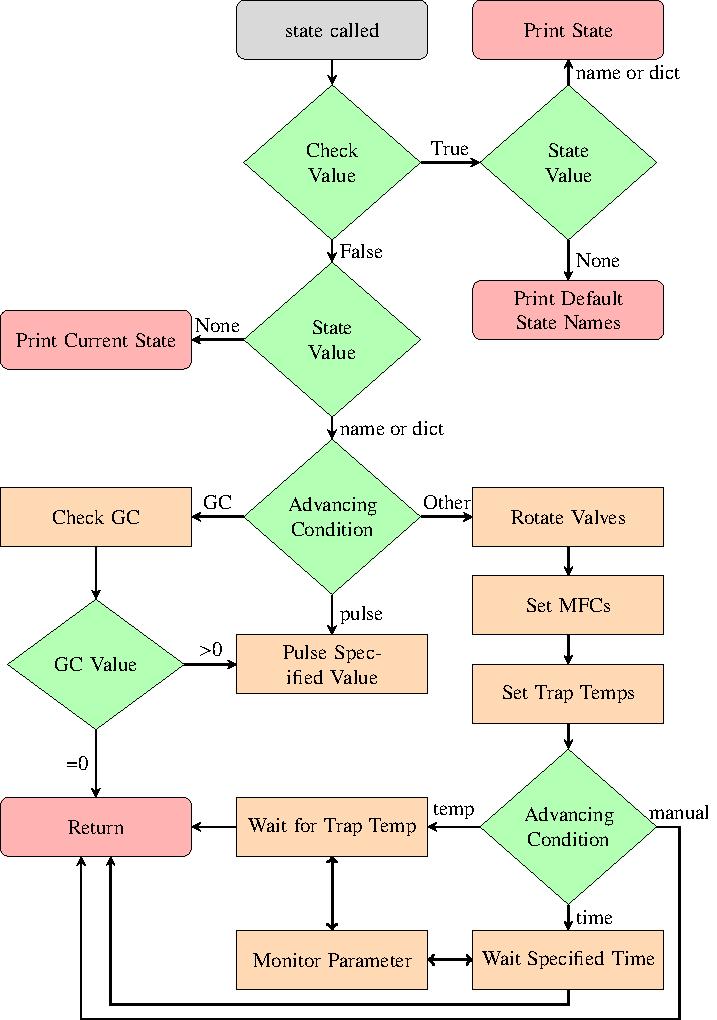
\includegraphics[width=0.9\linewidth]{tikz/state flow chart.pdf}
    \caption{State function flow chart detailing how individual controls are executed based on input conditions. Rounded rectangles with red backgrounds indicate exit conditions. Green diamonds are logic tests. Sharp rectangles with light orange backgrounds are processes that are executed prior to the next step.}
    \label{fig:state flow chart}
\end{figure}

\subsection{Methods}
Methods are a list of sequential states (dictionary objects) that are iterated over to perform a given task on the pre-concentration system. These are used to process samples, and perform maintenance. Methods are saved as a text files and saved in the \say{root/src/Methods/} folder. There are three functions associated with methods: \code{run\_method()}, \code{check\_method()}, and \code{standard\_run()}.

The \code{run\_method} function accepts a blank call, an integer, or a string. Typical operation will use a string input that simply specifies the file name of a method stored in the \say{Methods} folder. A blank call (i.e., \code{run\_method()} with list all methods saved in the Methods folder with an index. If an integer is provided, the indexed method from a blank call will be loaded and run. Method indices are not static and may change as new methods are added to or deleted from the Methods folder. Operators should only use an indexed call after checking which methods are available.

Methods generate errors mid-run, either for a process parameter being beyond what the system is capable of, or an invalid state is called within the sequence. Errors are handled within the scope of a method by first setting the pre-concentration system to the \say{off} state, and logging the error message in the method log. The system will then \code{raise} the error to terminate the method. \textbf{Warning:} the system defaulting to the \say{off} state only occurs when handling a system error. A system crash will not trigger any error handling while executing a state. This means there is no software fail-safe for code execution being terminated by the OS or power-loss.

Once a method has completed a run, it will automatically be logged in the \say{method log.txt} file that is located in the logs folders. Log files contain when the method was called, when it was completed, what method was used, and any notes associated with it. Notes can include state monitor results, or error messages that caused a method to fail.

%%%%%%%%%%%%%%%%%%%%%%%%%%%%%%%%%%%%%%%%%%%%%%%%%%%%%%%%%%%%%%%%%%%%%%%%%%%%
%%%%%%%%%%%%%%%%%%%%%%%%%%%%%% METHOD LOGGING %%%%%%%%%%%%%%%%%%%%%%%%%%%%%%
%%%%%%%%%%%%%%%%%%%%%%%%%%%%%%%%%%%%%%%%%%%%%%%%%%%%%%%%%%%%%%%%%%%%%%%%%%%%

There are a number of methods that were designs for regular operation of the pre-concentration system.

\begin{itemize}
    \item \textbf{direct inject} - This processes high concentration samples by using the trap by-pass plumbing as a sample trap. The connections between Valve 0 and Valve 1 function as a sample loop of \texttildelow 140 uL. The selected sample flushes the loop. Flow is disabled and given time to equilibrate with ambient pressure, and the sample is injected. This method triggers the GC.
    \item \textbf{change over flush} - Brief process to clear the line of a previous sample. The sampling line is evacuated and new sample gas flows through the system to prime the sample line. This method is automatically called when a method run switches sample port.
    \item \textbf{process sample} - This is simply the second half of the standard method. It is used when a sample is loaded, but something interrupts the method prior to injection. It proceeds from the back-flush steps of the standard method. This method triggers the GC.
    \item \textbf{bakeout} - backflush and bake out trap to remove anything left on the trap.
    \item \textbf{check heater} - Helper method to verify proper functionality of the system. Briefly back-flushes the trap, turns the heater on and verifies heat is applied. The heater is then turned off.
    \item \textbf{check mfc} - There is an automated version that verifies MFCs functionality. A manual version exists for the purpose of calibrating the backflush or sample MFC.
    \item \textbf{check valves} - Iterates by cycling each valve and checking with the operator to validate functionality.
\end{itemize}

\subsubsection{Creating a Custom Method}

The most user friendly way to create a custom method is with the \code{standard\_run()} function. This is the same function described in the command line interface (INSERT REFERENCE LINK) to modify the process parameters of the \say{standard} method. This function works by creating a copy of the standard method and modifying its parameters to match the input specifications. The default file name for a method created this way is \say{custom}, but a user can specify a file name. The function automatically saves the modified method and runs it by using \code{run\_method(file name)}. Custom methods created this way are the safest to run as it prevents users from creating a method with typos or invalid values. 

Advanced users may create a custom method by creating or directly editing the method text file. Text files are converted to python objects using \code{json.read}. There are some quirks about how json interprets files that is different from python. Some things to consider are that strings must always have full quotation marks, such as \say{string}. An error will occur if the file instead says 'string'. Errors will also occur with tailing commas, such as a dictionary with the following syntax that would not error in python:
\begin{center}
    \{\say{an integer}: 1,\\
    \say{a string}: \say{the string}\colorbox{yellow}{,}\}
\end{center}
Lastly, a key difference is that \code{None} values must be written as \code{Null}.

\code{check\_method} command is provided to help prevent errors that may occur while running a method, and to validate details of a method. New methods should always be checked before being run for the first time. A direct call with the sequence name will print how many state transitions there are, what their names are, and how long the method is expected to run. This is done by iterating through each state in a method and validating that each state will not generate an error, and logging all specified delays and timeouts. Delays determine the minimum run time, and the added timeouts estimate the maximum amount of time a method may require to complete. A method will also check if the GC remote is ever triggered during the method and print a warning if the GC is never triggered.


\subsection{Sequences}

Sequences are the highest level controls of the system. Sequences loop through method calls, similar to how methods loop through state calls. However, a sequence are intended to broaden the range of software control to allow for continuous operation of the pre-concentration system. The function is passed the name of the sequence to run, with an option for continuous operation:

\code{run\_sequence(sequence\_name, continuous=bool}

A continuously running sequence can be terminated at the completion of a method run by flipping the debug switch on the front panel to the on position.

Complete sequences are a list of sequence objects. Sequence objects are a custom defined dictionary that contain the following parameters:

\begin{table}[H]
    \centering
    \caption{Description of dictionary keys for sequences.}
    \begin{tabular}{l|p{0.5in}p{3in}p{1in}}
        Key         & Type      & Description   & Example\\
        \hline
        sample        & string    & Name of gas being measured & PDX Air\\
        method      & string      & Name of method to call    & 2000 mL sa\\
        repetition         & numeric   & Number of times to repeat method   & 24\\
        time         & numeric   & Total method time in minutes & 45\\
        on error   & string   & Specify how to handle errors & continue\\
    \end{tabular}
    \label{tab:sequence keys}
\end{table}

These parameters allow for selecting which stream to select, repeat a given method, and provide optional error handling if a method fails. The sample name field is passed as notes to the method, so that the method log will accurately reflect which sample was run at a given time.

\subsubsection{Autonomous Operation}
\label{auto operation}
Three bash scripts facilitate autonomous operation of the pre-concentration system: \say{day\_runner.sh}, monitor.sh, and check\_runner.sh.

day\_runner.sh initiates the pre-concentration system with a call to run a sequence continuously. This is wrapped with the \code{nohup} bash command which runs the script in the background on the Pi. \code{nohup} also logs everything that is printed to the terminal.

The other two scripts are not necessary to run, but helpful to successfully run the system. 
\code{monitor.sh} finds the most recently created \code{nohup} output file and monitors its output. This can be accessed from any connection to the Pi to see what it is doing. 
\code{check\_runner.sh} simply returns the process ID for the current running pre-concentration script. If there is an issue with the current running sequence, the process ID is needed to stop the sequence. Use the process ID to terminating the \code{nohup} script using the kill command: 
\code{kill -9 [process ID]}.

There are two advantages to running a \code{nohup} script: expanded logging, and background operation. Unlike methods, sequences do not have an automatic logging feature. Though each method run by the sequence is logged in the method's log, the nohup script will also log everything printed to the terminal. This can be useful for debugging any errors that may have occured. For background operation, the Raspberry Pi in the pre-concentration system is a headless module. This means that any active script relies on a stable connection with the controlling computer. A nohup script runs in the background and can be monitored from any connection. 

\pagebreak